\PassOptionsToPackage{dvipsnames}{xcolor} % https://tex.stackexchange.com/a/653721/258644
\documentclass[20pt, a0paper, portrait]{tikzposter}

% original template: https://rig.cs.luc.edu/~rig/home/tex/tikz/tikzposter-example.tex
%\usepackage{hyperref} % buggy: https://tex.stackexchange.com/questions/165846/incompatibility-between-tikzposter-class-and-microtype-package and https://bitbucket.org/surmann/tikzposter/issues/42/ctan-does-not-have-a-recent-version
\usepackage{url}
\usepackage{amsmath}
\usepackage{graphicx}
\usepackage{adjustbox}
\usepackage{twemojis}
\usepackage{mathrsfs} % \mathscr
\usepackage{multicol}
\usepackage{setspace} % \setstretch etc.

\usepackage{fontspec}
\setmonofont[Scale=MatchLowercase]{JuliaMono}
\newcommand{\emoji}[1]{{\setmainfont{Noto Color Emoji}[Renderer=Harfbuzz]{#1}}} % instead of \usepackage{emoji}

\usepackage{tikz}
\usetikzlibrary{positioning}
\usetikzlibrary{arrows}
\usetikzlibrary{arrows.meta}
\usetikzlibrary{trees}

\usepackage{tcolorbox}
\definecolor{codebg}{HTML}{F5F5F5}
%\definecolor{codefg}{HTML}{444444}
\definecolor{codeframe}{HTML}{DBDBDB}
\newtcolorbox{codeinbox}{
boxrule = 3pt,
boxsep = 8pt,
colback = codebg,
colframe = codeframe,
}
\newtcolorbox{codeoutbox}{
boxrule = 3pt,
boxsep = 8pt,
colback = white,
colframe = codeframe,
}

% https://tex.stackexchange.com/a/476488
% http://www.numdam.org/item/CG_1998___28-29_158_0.pdf
\usepackage{fancyvrb}
\fvset{formatcom=\setlength{\lineskip}{0pt}}
\begin{SaveVerbatim}{code1}
using SymBoltz, Unitful, UnitfulAstro, ModelingToolkit, ForwardDiff, Plots
M = ΛCDM()
\end{SaveVerbatim}
\begin{SaveVerbatim}{code2}
equations(M.G)
\end{SaveVerbatim}
\begin{SaveVerbatim}{code3}
params = Dict(
    M.γ.T₀ => 2.7,  M.ν.Neff => 3.0,  M.g.h      => 0.7,
    M.c.Ω₀ => 0.27, M.b.Ω₀   => 0.05, M.b.rec.Yp => 0.25,
    M.I.As => 2e-9, M.I.ns   => 0.95, M.h.m      => 0.06u"eV/c^2/kg"+0
)
prob = CosmologyProblem(M, params) # symbolic-to-numeric compilation
\end{SaveVerbatim}
\begin{SaveVerbatim}{code4}
ks = [1e-2, 1e-1, 1e0] / u"Mpc" # wavenumbers
sol = solve(prob, ks) # solution object
p1 = plot(sol, ks, log10(M.g.a), [M.g.Φ, M.g.Ψ]) # use included plot recipe

ks = 10 .^ range(-3, 0, length=200) / u"Mpc" # wavenumbers for matter power spectrum
function Pk(θ) # define P(k; θ) as a function of some independent parameters θ
    newprob = remake(prob, Dict(M.c.Ω₀ => θ[1], M.b.Ω₀ => θ[2], M.g.h => θ[3]))
    sol = solve(newprob, ks; ptopts = (reltol = 1e-3,))
    return spectrum_matter(sol, ks)
end
θ = [params[M.c.Ω₀], params[M.b.Ω₀], params[M.g.h]]
Ps = Pk(θ)
dlgPs = ForwardDiff.jacobian(lgθ -> log10.(Pk(10 .^ lgθ) / u"Mpc^3"), log10.(θ))
p2 = plot(ks, Ps; xlabel="k", ylabel="P", xaxis=:log, yaxis=:log, label=nothing)
p3 = plot(ks, dlgPs; xlabel="k", xaxis=:log, label="∂(lg P)/∂(lg ".*["Ωc0)" "Ωb0)" "h)"])

p = plot(p1, p2, p3; size=(1600,400), layout=(1,3), margin=(8,:mm), bg=false, grid=false)
\end{SaveVerbatim}
\begin{SaveVerbatim}{code5}
using SymBoltz: t, k, ϵ, D, O # use variables, derivative and perturbation operator
g = M.g # get metric of original model
pars = @parameters w₀ wₐ cₛ² Ω₀ # create parameters
vars = @variables ρ(t) P(t) w(t) δ(t) θ(t) σ(t) # create variables
eqs = [ # specify equations
    O(1)(w ~ w₀ + wₐ * (1 - g.a)) # equation of state
    O(1)(ρ ~ 3/(8*Num(π))*Ω₀ * g.a^(-3*(1+w₀+wₐ))) # energy density
    O(1)(P ~ w * ρ) # pressure
    O(ϵ)(D(δ) ~ -(1+w)*(θ-3*g.Φ) - 3*g.ℰ*(cₛ²-w)*δ) # overdensity
    O(ϵ)(D(θ) ~ -g.ℰ*(1-3*w)*θ - D(w)/(1+w)*θ + k^2*(cₛ²/(1+w)*δ + g.Ψ)) # momentum
    O(ϵ)(σ ~ 0) # shear stress
]
initialization_eqs = [ # initial conditions
    O(ϵ)(δ ~ -3/2 * (1+w) * g.Ψ)
    O(ϵ)(θ ~ 1/2 * (k^2/g.ℰ) * g.Ψ)
]
description = "w₀wₐ (CPL) dynamical dark energy"
@named X = ODESystem(eqs, t, vars, pars; initialization_eqs, description)

M = ΛCDM(Λ = X; name = :w₀wₐCDM) # recreate ΛCDM model, but replace CC by w0wa
params = merge(params, Dict(M.X.w₀ => -0.9, M.X.wₐ => 0.2, M.X.cₛ² => 1.0))
prob = CosmologyProblem(M, params) # create new problem
sol = solve(prob, ks) # solve new problem; then continue as before ...
\end{SaveVerbatim}
\begin{SaveVerbatim}{code6}
hierarchy(M; describe=true) # view hierarchical structure of model components
\end{SaveVerbatim}
\begin{SaveVerbatim}{out6}
ΛCDM: Standard cosmological constant and cold dark matter cosmological model
├─ g: Spacetime FLRW metric in Newtonian gauge
├─ G: General relativity gravity
├─ γ: Photon radiation
├─ ν: Massless neutrinos
├─ c: Cold dark matter
├─ b: Baryonic matter
│  └─ rec: Baryon-photon recombination thermodynamics (RECFAST)
├─ h: Massive neutrino
├─ Λ: Cosmological constant
└─ I: Harrison-Zel'dovich inflation
\end{SaveVerbatim}

\title{\huge SymBoltz.jl: symbolic-numeric, approximation-free and differentiable Boltzmann code}
\author{\huge Herman Sletmoen -- University of Oslo}
\institute{}
\titlegraphic{\includegraphics[width=\textwidth]{logo.png}\\\tiny \textcolor{brown}{\textbf{Dall-E:} Albert Einstein (with messy hair) and Ludwig Boltzmann (with long beard) happily solving equations together on a computer. Cartoon. Old style.}}

% adapted from /usr/share/texlive/texmf-dist/tex/latex/tikzposter/tikzposterColorstyles.tex
\definecolorstyle{MyColorStyle}{
    % Define default colors
    % GrayBlueYellow
    \definecolor{colorOne}{HTML}{F5F5F5} % gray
    \definecolor{colorTwo}{HTML}{0066A8} % blue
    \definecolor{colorThree}{HTML}{f1a73c}
    %\definecolor{colorThree}{HTML}{FCE565} % yellow
}{
     % Background Colors
    \colorlet{backgroundcolor}{colorOne}
    \colorlet{framecolor}{colorTwo}
    % Title Colors
    \colorlet{titlefgcolor}{black}
    \colorlet{titlebgcolor}{colorThree}
    % Block Colors
    \colorlet{blocktitlebgcolor}{colorThree}
    \colorlet{blocktitlefgcolor}{black}
    \colorlet{blockbodybgcolor}{white}
    \colorlet{blockbodyfgcolor}{black}
    % Innerblock Colors
    \colorlet{innerblocktitlebgcolor}{colorThree}
    \colorlet{innerblocktitlefgcolor}{black}
    \colorlet{innerblockbodybgcolor}{white}
    \colorlet{innerblockbodyfgcolor}{black}
    % Note colors
    \colorlet{notefgcolor}{black}
    \colorlet{notebgcolor}{colorThree!70!white}
    \colorlet{notefrcolor}{colorThree}
 }

%\useblockstyle[roundedcorners=10,linewidth=0pt]{Default} % must comment \usetheme and \usecolorstyle
%\usetheme{metropolis}
\usecolorstyle{MyColorStyle}
\usetitlestyle{Filled} % title covers width
\useblockstyle[bodyverticalshift=-1cm]{TornOut} % Default / Basic / Minimal / Envelope / Corner / Slide / TornOut
%\useinnerblockstyle{Table}
%\usecolorstyle[colorPalette=BrownBlueOrange]{Germany}

% https://tex.stackexchange.com/a/167527
\makeatletter
\renewcommand\TP@maketitle{%
    \begin{minipage}{0.15\linewidth}
        \centering
        \@titlegraphic
    \end{minipage}%
    \hfill%
   \begin{minipage}{0.85\linewidth}
        \centering
        \color{titlefgcolor}
        {\bfseries \Huge \sc \@title \par}
        \vspace*{1.5em}
        {\LARGE \@author \par}%
        %\vspace*{1em}
        %{\LARGE \@institute}
    \end{minipage}%
}
% https://tex.stackexchange.com/a/315059/258644
\renewenvironment{tikzfigure}[1][]{
  \def \rememberparameter{#1}
  %\vspace{10pt}
  %\refstepcounter{figurecounter}
  \begin{center}
  }{
    \setstretch{0.9}%
    \\[5pt]%
    {\small \rememberparameter}
  \end{center}
}
\makeatother

\begin{document}
\maketitle

\begin{columns}

\column{.50}

\block[]{New features}{
    \begin{itemize}
    \item \textbf{Symbolic-numeric architecture:} Represents equations symbolically, and generates fast numerical code from them. Combines the powers of symbolic equation modeling and efficient numerical computing into one integrated framework for easier cosmological modeling.
    \item \textbf{Modular physical structure:} Structured around physical components (e.g. gravity and particle species). Easily replace one component with another without modifying the entire model. Build a library of small self-contained physical components, and join any of them into full cosmological models. Accomodates extended models in a way that scales in model space. Computational stages (background, perturbations, \ldots) should be detected automatically from interdependencies between the equations.
    \item \textbf{Approximation-free:} Integrates the full (stiff) Einstein-Boltzmann equations at all times with a wide selection of modern (implicit) solvers. No tight coupling, ultra-relativistic, radiation streaming or other approximations. Makes code simpler and extended models easier to implement.
    \item \textbf{Differentiable:} Compute $\partial(\mathrm{output})/\partial(\mathrm{input})$ for any input and output (e.g. $\partial P(k) / \partial \Omega_{m0}$) with automatic differentiation (exact numerical differentiation of arbitrarily complicated functions). Important for accurate Jacobians for implicit ODE solvers, and for gradient-based numerical methods, like efficient many-parameter inference methods (e.g. HMC/NUTS), machine learning and optimization problems.
    \item \textbf{Convenient:} Eliminates chores one must do when extending traditional codes. Focus on \emph{modeling}.
    \end{itemize}
}

\block[]{Architecture}{
    SymBoltz.jl relies on ModelingToolkit.jl for symbolic modeling and conversion to efficient numerical code, and on DifferentialEquations.jl for ODE integration and access to stiff solvers.
    We want to take advantage of and contribute to this growing symbolic-numeric modeling library for the benefit of all sciences.

    \begin{minipage}{0.49\linewidth}
    \bigskip
    \begin{tikzfigure}[
        \textbf{Structure:}
        For optimal modularity, SymBoltz is structured according to the \emph{physical} layout of cosmological models.
        Components can be added, replaced or modified independently.
        The best \emph{computational} structure (e.g. background $\rightarrow$ thermodynamics $\rightarrow$ perturbations) is found internally.
    ]
    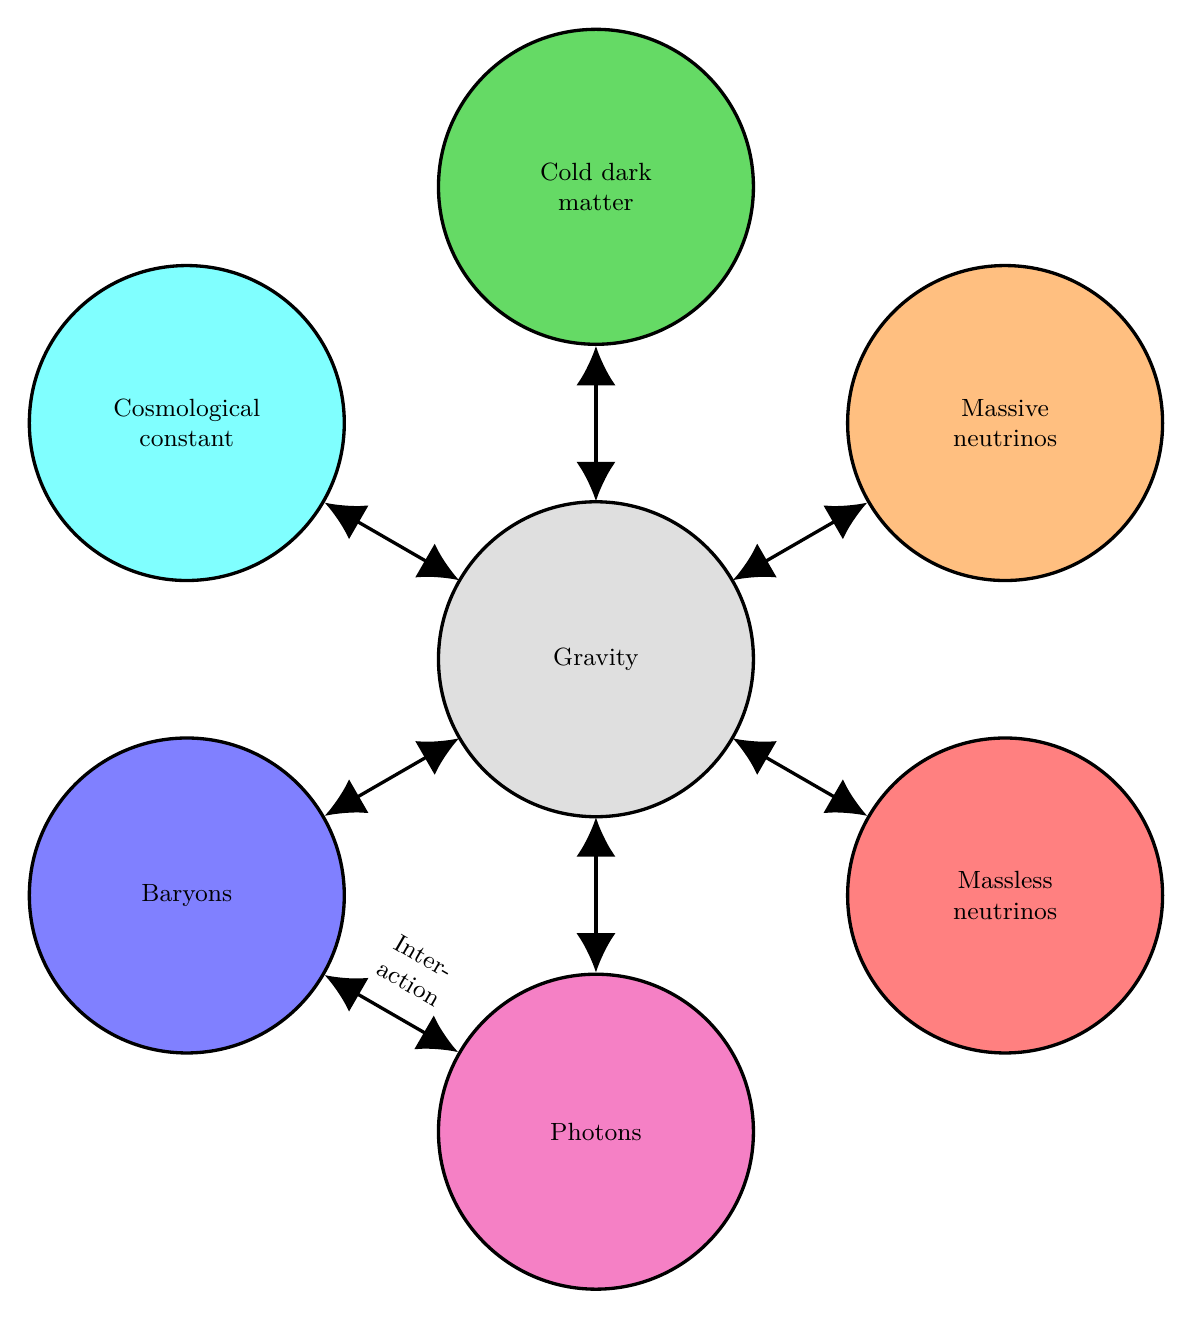
\begin{tikzpicture}[
        font=\small,
        comp/.style = {draw, circle, fill=gray, minimum size = 4cm, align=center},
        grow cyclic,
        level 1/.append style = {level distance = 6cm, sibling angle = 60},
        interaction/.style = {{Latex[width=5mm,length=5mm]}-{Latex[width=5mm,length=5mm]}, very thick},
        ]
        \node[comp, fill=lightgray!50] (grav) {Gravity} [interaction]
        child { node[comp, fill=blue!50] (bar) {Baryons}}
        child { node[comp, fill=magenta!50] (pho) {Photons}}
        child { node[comp, fill=red!50] (neu) {Massless\\neutrinos}}
        child { node[comp, fill=orange!50] (mneu) {Massive\\neutrinos}}
        child { node[comp, fill=LimeGreen!75] (cdm) {Cold dark\\matter}}
        child { node[comp, fill=Cyan!50] (cc) {Cosmological\\constant}};
        \draw[interaction] (bar) -- node[above=2mm, sloped, align=center] {Inter-\\action} (pho);
    \end{tikzpicture}
    \end{tikzfigure}
    \end{minipage}%
    \hfill%
    \begin{minipage}{0.49\linewidth}
    \bigskip
    \begin{tikzfigure}[
        \textbf{Synergy of features:}
        For example, automatic differentiation helps to calculate the ODE Jacobian $J$ robustly, which is needed by implicit solvers to integrate ODEs without approximations, which makes it easier to write down models in a simple symbolic form, which can be used to detect the sparsity pattern of $J$, which in turn increases the efficiency of automatic differentiation, \ldots.
        This makes a stronger self-reinforcing design.
    ]
    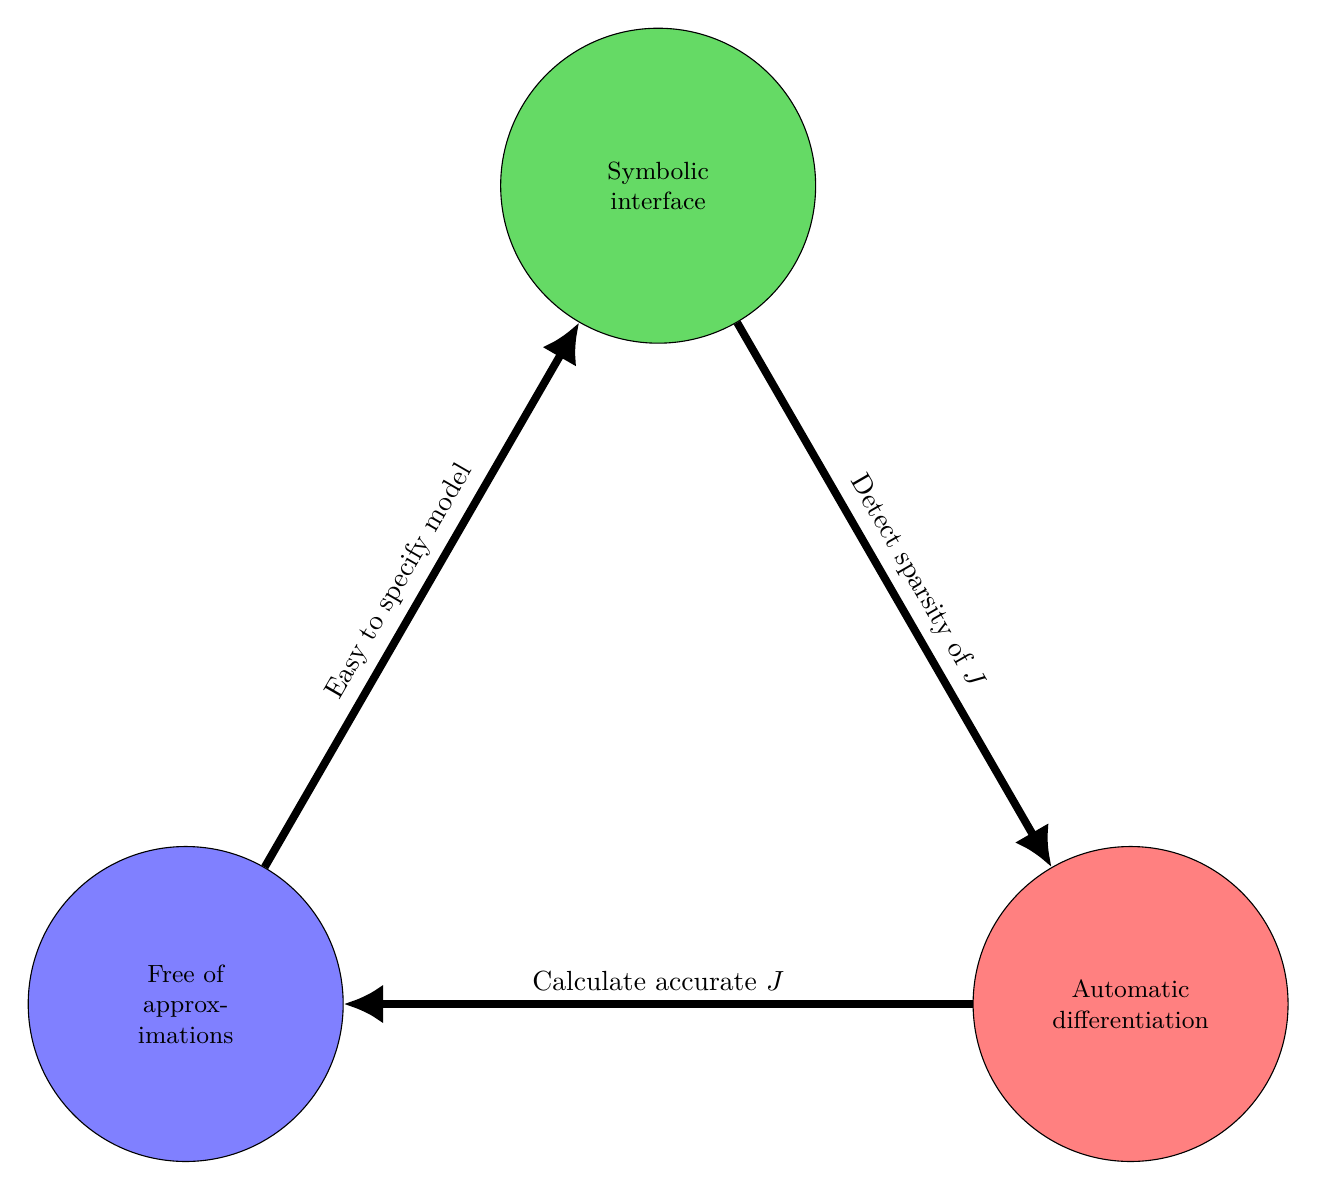
\begin{tikzpicture}[
        pillar/.style={circle, draw, minimum size=4cm, align=center, font=\small},
        joiner/.style={midway, sloped, black, font=\normalsize},
        arrow/.style={-{Latex[width=5mm,length=5mm]}, line width=1mm, black},
    ]
    \node[pillar, fill=LimeGreen!75] (sym) at (0:0cm) {Symbolic\\interface};
    \node[pillar, fill=blue!50] (app) at (240:12cm) {Free of\\approx-\\imations};
    \node[pillar, fill=red!50] (dif) at (300:12cm) {Automatic\\differentiation};
    \draw[arrow] (sym.300) -- node[joiner, above] {Detect sparsity of $J$} (dif.120);
    \draw[arrow] (dif.180) -- node[joiner, above] {Calculate accurate $J$} (app.0);
    \draw[arrow] (app.60) -- node[joiner, above] {Easy to specify model} (sym.240);
    \end{tikzpicture}
    \end{tikzfigure}
    \end{minipage}
}

\block[bodyverticalshift=-1.75cm]{Goals}{
    \begin{itemize}
        \item \textbf{Create an integrated symbolic-numeric Einstein-Boltzmann modeling \emph{environment}} (not ``just'' a solver). Grow into a full linear + non-linear framework including $N$-body simulations?
        \item \textbf{Make it easier for modelers to build modified models} by avoiding complicating approximations and using mixed symbolic-numeric computing to automate chores and provide helpful utilities.
                The goal is to \textbf{let the modeler simply write down \emph{one single set} of Einstein-Boltzmann equations for their cosmological model}.
                SymBoltz should \emph{automatically} detect the structure in the equations, split it up into stages (background $\rightarrow$ thermodynamics $\rightarrow$ perturbations $\rightarrow$ \ldots), spline functions between each stage, generate suitable initial conditions, change to a suitable independent variable, generate code and solve the model, compute and plot derived quantities, and so on.
        \item \textbf{Design a structure that is modular in terms of \emph{physical} components} and scales better in model space.
                Rethink the traditional Boltzmann solver layout to avoid duplicating large monolithic codes for every combination of models/extensions, which often grow into mutually incompatible forks.
        \item \textbf{Enable powerful gradient-based optimization/MCMC methods} (e.g. HMC/NUTS) by being fast and differentiable.
                Important for many-parameter inference from next-generation surveys!
    \end{itemize}
}

\block[bodyverticalshift=-1.75cm]{Implementation status (\textcolor[HTML]{7CB342}{complete}, \textcolor[HTML]{FFCC32}{in progress} and \textcolor[HTML]{F44336}{planned})}{ % colors from dropper tool on emojis
    \small
    \begin{multicols}{3}
    \emoji{🟩} Baryons + photons (RECFAST recombo.) \\
    \emoji{🟩} Cold dark matter \\
    \emoji{🟩} Massless and massive neutrinos \\
    \emoji{🟩} Cosmological constant \\
    \emoji{🟨} Quintessence \\
    \emoji{🟩} $w_0 w_a$ dark energy \\
    \emoji{🟩} General Relativity \\
    \emoji{🟨} Brans-Dicke gravity \\
    \emoji{🟨} Curved geometry \\
    \emoji{🟩} Symbolic interface \\
    \emoji{🟩} Approximation-free (no TCA, RSA, UFA, \ldots) \\
    \emoji{🟩} Forward-mode automatic differentiation \\ 
    \emoji{🟩} Matter power spectrum \\
    \emoji{🟩} CMB power spectrum (TT, TE, EE) \\
    \emoji{🟨} Automatic stage separation ($\text{backgr.} \rightarrow \text{pert.}$) \\
    \emoji{🟩} Automatic splining of ODE unknowns \\
    \emoji{🟩} Automatic recomputation of ODE observeds \\
    \emoji{🟩} Automatic interpolation in $(\tau, k)$ of all variables \\
    \emoji{🟨} Automatic change of variables ($\frac{\mathrm{d}}{\mathrm{d}\tau} \rightarrow \frac{\mathrm{d}}{\mathrm{d \ln a}}$) \\
    \emoji{🟨} Automatic series expansion of initial conditions \\
    \emoji{🟩} Automatic parameter assignment hooks \\
    \emoji{🟩} Shooting method for boundary conditions \\
    \emoji{🟩} Plot recipes (for convenient inspection) \\
    \emoji{🟨} Performance (isolate symbolics from numerics) \\
    \emoji{🟩} Extensive documentation pages \\
    \emoji{🟩} Continuous integration and testing \\
    \emoji{🟩} Comparison with \textsc{class} for ΛCDM \\
    \emoji{🟨} Non-linear: \textsc{halofit}/\textsc{hmcode} \\
    \emoji{🟥} Non-linear: generate $N$-body problems \\
    \emoji{🟥} Reverse-mode automatic differentiation \\
    \emoji{🟥} Automatic unit conversion utilities \\
    \emoji{🟥} Symbolic tensor manipulation \\
    \emoji{🟥} GPU parallellization \\
    \emoji{🟥} Better representation of interactions \\
    \emoji{🟨} Publication paper \\
    \emoji{⬛} \textbf{Ideas/contributions are very welcome!}
    \end{multicols}
}

% https://tex.stackexchange.com/a/183867
\block[bodyverticalshift=-2.0cm]{\huge Try it! Feedback?}{
\noindent
\begin{minipage}{0.25\linewidth}
    \includegraphics[width=\linewidth]{../qr.png}
\end{minipage}%
\hfill%
\begin{adjustbox}{valign=c}%
\begin{minipage}{0.75\linewidth}
    \LARGE Easy installation and extensive documentation:
    \begin{quote}
        \LARGE \textcolor{blue}{\url{github.com/hersle/SymBoltz.jl}}
    \end{quote}
    SymBoltz.jl is in development. Feedback is appreciated! \\
    Interested? Questions? Suggestions? Contributions?\\
    \textbf{Star it! \emoji{🌟} Open an issue or pull request! \emoji{👷}}
\end{minipage}
\end{adjustbox}
}

\column{.50}

\block{Code demonstration (as of latest version)}{
    Install and launch \texttt{julia}. Load some packages and build a standard ΛCDM model:
    \begin{codeinbox}
    \UseVerbatim{code1}
    \end{codeinbox}
    This is a purely \emph{symbolic} model representation.
    It can be interactively inspected and modified.
    Every physical component lives in a 1-letter subcomponent:
    the metric $g$, gravity $G$, photons $\gamma$, massless neutrinos $\nu$, massive neutrinos $h$, cold dark matter $c$, baryons $b$ and the cosmological constant $\Lambda$.
    There is no separation between the background and perturbations here.
    For example, we can view the equations in the gravity component:
    \begin{codeinbox}
    \UseVerbatim{code2}
    \end{codeinbox}
    \begin{align}
        \frac{\mathrm{d} a\left( t \right)}{\mathrm{d}t} &= \sqrt{\frac{8}{3} \left( a\left( t \right) \right)^{4} \rho\left( t \right) \pi} \\
        \Delta\left( t \right) &= \frac{\mathrm{d}}{\mathrm{d}t} \frac{\mathrm{d} a\left( t \right)}{\mathrm{d}t} + \frac{ - \left( \frac{\mathrm{d} a\left( t \right)}{\mathrm{d}t} \right)^{2} \left( 1 + \frac{ - 3 P\left( t \right)}{\rho\left( t \right)} \right)}{2 a\left( t \right)} \\
        \frac{\mathrm{d} \Phi\left( t \right)}{\mathrm{d}t} \epsilon &= \left( \frac{ - k^{2} \Phi\left( t \right)}{3 \mathscr{E}\left( t \right)} + \frac{ - \frac{4}{3} \left( a\left( t \right) \right)^{2} \mathtt{\delta\rho}\left( t \right) \pi}{\mathscr{E}\left( t \right)} - \mathscr{E}\left( t \right) \Psi\left( t \right) \right) \epsilon \\
        k^{2} \left(  - \Psi\left( t \right) + \Phi\left( t \right) \right) \epsilon &= 12 \left( a\left( t \right) \right)^{2} \Pi\left( t \right) \pi \epsilon
    \end{align}
    Next, we can map parameters to some values and compile a \emph{numerical} problem from the symbolic system.
    This is where ``the magic happens'': the symbolic system is checked for consistency, broken down into background and perturbation stages, splines are set up to pass the solution of one stage to the next, and so on.
    \begin{codeinbox}
    \UseVerbatim{code3}
    \end{codeinbox}
    Now we can solve the problem.
    The resulting solution object can be indexed with any symbolic expression to get its numerical value (it is automatically computed from the ODE state vector).
    We can also calculate derived quantities, like the matter power spectrum.
    Gradients can be obtained with automatic differentiation.
    \begin{codeinbox}
    \UseVerbatim{code4}
    \end{codeinbox}
    \includegraphics[width=\linewidth]{plot.pdf}
    Finally, let us implement a new species for $w_0 w_a$ dark energy (as if it is not already available in the code).
    \begin{codeinbox}
    \UseVerbatim{code5}
    \end{codeinbox}
    We only had to write down the equations; not modify any internal code.
    Everything (e.g. background and perturbation quantities) is defined in the same place to encourage modularity.
    Similar implementations in other codes can require many more changes and in many different places, effectively forking and fragmenting the code.
    Proceed as before to inspect and solve the new model. See the documentation for more examples!
    %\includesvg[width=\linewidth]{uio-logo.svg}
}

\end{columns}

\end{document}
